%% generato automaticamente da tools/build_tex.py --- non modificare
\chapter{Il seno cardinale e il suo gemello}
\label{cap:cosinc}
\quaderno{cosinc.dfw}{14 Nov 2010}{29}

Novembre 2010. Il quaderno studia una sola funzione, $\dfrac{(-1)^x-1}{\pi x}$, e la ragione per cui è interessante sta tutta nella scrittura $(-1)^x$. Con la determinazione principale — quella dichiarata nell'intestazione del file — si ha $(-1)^x=\mathrm{e}^{\mathrm{i}\pi x}$, e la funzione diventa $\dfrac{\mathrm{e}^{\mathrm{i}\pi x}-1}{\pi x}$: un oggetto complesso la cui parte immaginaria è il seno cardinale e la cui parte reale è una funzione molto simile ma con proprietà opposte. Il titolo del file mette insieme le due parole.

\section{L'unità immaginaria come rapporto di derivate}

Le prime tredici righe girano attorno a un modo di far comparire $\mathrm{i}$: derivare $(-1)^{kx}$ e dividere per il risultato atteso.

\begin{espr}{1}{User}{}
\[
\frac{\left(1 + \mathrm{i}\, \tan\!\left(t\right)\right)^{2}}{1 + \tan^{2}\!\left(t\right)}
\]
\end{espr}
Il quadrato del numero $1+\mathrm{i}\tan t$ normalizzato: è $\mathrm{e}^{2\mathrm{i}t}$, per la parametrizzazione razionale del cerchio.

\begin{espr}{2}{User}{}
\[
\operatorname{sgn}^{2}\!\left(1 + \mathrm{i}\, \tan\!\left(t\right)\right)
\]
\end{espr}
La stessa cosa scritta con la funzione segno complessa.

\begin{espr}{3}{User}{}
\[
1 + \mathrm{i}\, \tan\!\left(t\right)
\]
\end{espr}
Il numero non normalizzato.

\begin{espr}{4}{User}{}
\[
1 + \tan^{2}\!\left(\pi\, t\right)
\]
\end{espr}
Il denominatore della normalizzazione, con argomento $\pi t$.

\begin{espr}{5}{User}{}
\[
1^{x}
\]
\end{espr}
L'unità elevata a qualunque esponente: la riga che introduce il tema delle potenze a base costante.

\begin{espr}{6}{User}{}
\[
\frac{\frac{\mathrm{d}}{\mathrm{d}x}\!\left[\left(-1\right)^{x}\right]}{\pi\, \left(-1\right)^{x}}
\]
\end{espr}
La derivata di $(-1)^x$ divisa per $\pi(-1)^x$: vale $\mathrm{i}$.

\begin{espr}{7}{User}{}
\[
\frac{\frac{\mathrm{d}}{\mathrm{d}x}\!\left[\left(-1\right)^{2\, x}\right]}{2\, \pi\, \left(-1\right)^{2\, x}}
\]
\end{espr}
Con esponente doppio, e il fattore $2\pi$ al denominatore: ancora $\mathrm{i}$.

\begin{espr}{8}{User}{}
\[
\frac{\frac{\mathrm{d}}{\mathrm{d}x}\!\left[\left(-1\right)^{3\, x}\right]}{3\, \pi\, \left(-1\right)^{3\, x}}
\]
\end{espr}
Con esponente triplo.

\begin{espr}{9}{User}{}
\[
\frac{\frac{\mathrm{d}}{\mathrm{d}x}\!\left[\left(-1\right)^{k\, x}\right]}{k\, \pi\, \left(-1\right)^{k\, x}}
\]
\end{espr}
Il caso generale: il rapporto vale $\mathrm{i}$ per ogni $k$.

\begin{espr}{10}{User}{}
\[
\frac{1}{x}\, \ln\!\left(x\right)
\]
\end{espr}
Il logaritmo diviso per l'argomento, annotato di passaggio.

\begin{espr}{11}{User}{}
\[
\lim_{h \to 0} \frac{\left(-1\right)^{h} - 1}{\pi\, h}
\]
\end{espr}
Lo stesso risultato come rapporto incrementale in zero.

\begin{espr}{12}{User}{}
\[
\left(\frac{\left(-1\right)^{h} - 1}{\pi\, h}\right)^{2}
\]
\end{espr}
Il suo quadrato, che vale $-1$.

\begin{espr}{13}{User}{}
\[
\frac{\left(-1\right)^{h} - 1}{\pi\, h}
\]
\end{espr}
Il rapporto incrementale prima del passaggio al limite: è la funzione che il quaderno studierà per il resto delle pagine.


Il meccanismo delle righe $\#6$--$\#9$ è questo: se $(-1)^{kx}=\mathrm{e}^{\mathrm{i}k\pi x}$, la sua derivata vale $\mathrm{i}k\pi\,\mathrm{e}^{\mathrm{i}k\pi x}$, e dividendo per $k\pi\,(-1)^{kx}$ resta esattamente $\mathrm{i}$, per ogni $k$. Quattro righe per il caso $k=1,2,3$ e poi il caso generale: è il modo in cui questi quaderni verificano una regolarità prima di enunciarla.

La riga $\#11$ ottiene lo stesso risultato per un'altra strada, come rapporto incrementale: $\lim_{h\to0}\frac{\mathrm{e}^{\mathrm{i}\pi h}-1}{\pi h}=\mathrm{i}$, che è la derivata in zero della stessa funzione. Questa volta il limite è genuinamente $\mathrm{i}$ e non una convenzione di scrittura — a differenza di quanto accadeva in \dfw{j.dfw} (capitolo~\ref{cap:j}), dove la stessa domanda era stata posta a un rapporto che tende a zero. Fra i due quaderni passano sedici mesi.

\section{La serie e le sue due parti}

Il cuore del quaderno. Si sviluppa in serie la funzione e si separano parte reale e parte immaginaria.

\begin{espr}{14}{User}{}
\[
\frac{\mathrm{i}^{n + 1}\, \left(\pi\, x\right)^{n}}{\left(n + 1\right)!}
\]
\end{espr}
Il termine generale dello sviluppo in serie.

\begin{espr}{15}{User}{}
\begin{align*}
& \operatorname{Im}\!\left(\sum_{n=0}^{+\infty} \frac{\mathrm{i}^{n + 1}\, \left(\pi\, x\right)^{n}}{\left(n + 1\right)!}\right) \\
=\;& \frac{\sin\!\left(\pi\, x\right)}{\pi\, x}
\end{align*}
\end{espr}
La parte immaginaria della somma è il seno cardinale.

\begin{espr}{16}{User}{}
\begin{align*}
& \operatorname{Re}\!\left(\sum_{n=0}^{+\infty} \frac{\mathrm{i}^{n + 1}\, \left(\pi\, x\right)^{n}}{\left(n + 1\right)!}\right) \\
=\;& \frac{\cos\!\left(\pi\, x\right) - 1}{\pi\, x}
\end{align*}
\end{espr}
La parte reale è il suo gemello, con il coseno al posto del seno.

\begin{figure}[htbp]
  \centering
  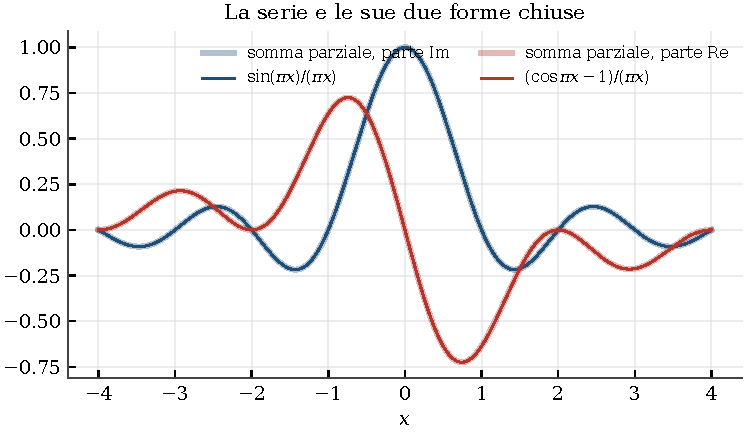
\includegraphics[width=0.86\linewidth]{../figures/cosinc_serie.pdf}
  \caption{La somma parziale della serie della riga $\#14$ (tratto spesso) confrontata con le due forme chiuse delle righe $\#15$ e $\#16$. Quaranta termini bastano a coprire l'intervallo mostrato.}
  \label{fig:cosinc_serie}
\end{figure}
\begin{espr}{17}{User}{}
\[
\frac{1 - \cos\!\left(\pi\, x\right)}{\pi\, x}
\]
\end{espr}
La stessa funzione con il segno cambiato, nella forma che verrà integrata.

\begin{figure}[htbp]
  \centering
  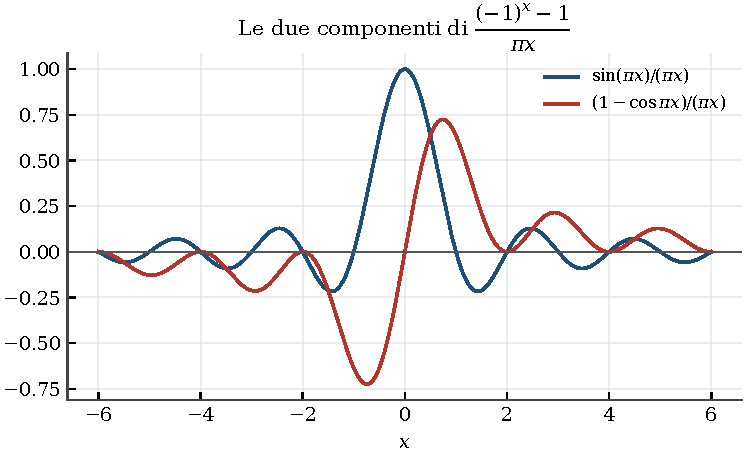
\includegraphics[width=0.86\linewidth]{../figures/sinc_cosinc.pdf}
  \caption{Le due componenti. Entrambe decrescono come $1/x$, ma il seno cardinale cambia segno a ogni intero e le sue aree si compensano, mentre l'altra resta positiva e la sua coda diverge.}
  \label{fig:sinc_cosinc}
\end{figure}

Lo sviluppo è immediato una volta riconosciuto l'esponenziale:
\[
  \frac{\mathrm{e}^{\mathrm{i}\pi x}-1}{\pi x}
  =\frac{1}{\pi x}\sum_{m\ge1}\frac{(\mathrm{i}\pi x)^m}{m!}
  =\sum_{n\ge0}\frac{\mathrm{i}^{\,n+1}(\pi x)^n}{(n+1)!},
\]
che è esattamente il termine generale della riga $\#14$. La parte immaginaria della somma è $\sin(\pi x)/(\pi x)$, cioè il seno cardinale normalizzato; la parte reale è $\left(\cos(\pi x)-1\right)/(\pi x)$. Le righe $\#15$ e $\#16$ affermano proprio questo, e la verifica numerica le conferma.

\section{Due integrali che si comportano in modo opposto}

Qui il quaderno confronta le due componenti sotto integrale su tutta la retta, e trova una differenza radicale. Su una delle due, però, Derive dà una risposta che va guardata con attenzione.

\begin{espr}{18}{User}{}
\[
2\, \int_{0}^{+\infty} \frac{1 - \cos\!\left(\pi\, x\right)}{\pi\, x} \,\mathrm{d}x
\]
\end{espr}
L'integrale su tutta la semiretta positiva, raddoppiato per simmetria.

\begin{espr}{19}{User}{}
\[
\int_{-+\infty}^{+\infty} \frac{\sin\!\left(\pi\, x\right)}{\pi\, x} \,\mathrm{d}x = 1
\]
\end{espr}
L'integrale del seno cardinale: vale esattamente uno. È l'integrale di Dirichlet.

\begin{espr}{20}{User}{}
\[
2\, \int_{0}^{+\infty} \frac{1 - \cos\!\left(\pi\, x\right)}{\pi\, x} \,\mathrm{d}x = 11.53414128
\]
\end{espr}
Il valore restituito per l'altra componente. L'integrale però diverge logaritmicamente: il numero è l'effetto di un troncamento della quadratura numerica intorno a $x\approx10^7$.

\begin{espr}{21}{User}{}
\[
\frac{11.53414128}{2}
\]
\end{espr}
La metà del valore precedente.

\begin{espr}{22}{User}{\verificata}
\[
\frac{11.53414128}{2} = 5.76707064
\]
\end{espr}
Che eredita lo stesso problema.

\begin{espr}{23}{User}{}
\[
\frac{\cos\!\left(\pi\, x\right) - 1}{\pi\, x}
\]
\end{espr}
La componente reale scritta con il segno opposto.

\begin{espr}{24}{User}{}
\[
\int \frac{1 - \cos\!\left(\pi\, x\right)}{\pi\, x} \,\mathrm{d}x
\]
\end{espr}
Il suo integrale indefinito.

\begin{espr}{25}{Int(User,x)}{}
\[
\int \frac{\sin\!\left(\pi\, x\right)}{\pi\, x} \,\mathrm{d}x
\]
\end{espr}
E quello del seno cardinale, che è il seno integrale.


Il seno cardinale è integrabile in senso improprio e la riga $\#19$ dà il valore corretto: $\int_{-\infty}^{+\infty}\frac{\sin\pi x}{\pi x}\,\mathrm{d}x=1$. È l'integrale di Dirichlet, e vale esattamente uno grazie alla normalizzazione con $\pi$.

L'altra componente non è integrabile. Per $x$ grande $\left(1-\cos\pi x\right)/(\pi x)$ oscilla attorno a $1/(\pi x)$, la cui coda diverge logaritmicamente: l'integrale cresce come $\frac{1}{\pi}\ln R$ e non ha limite. Il valore $11{,}53414128$ della riga $\#20$ non è dunque il valore dell'integrale, ma il risultato di una quadratura numerica troncata. Rifacendo il conto si trova che il troncamento corrisponde a un estremo superiore di circa $10^7$: portandolo a $10^9$ il risultato sale a $14{,}4$, e continua a crescere. È il caso in cui un sistema di calcolo restituisce un numero dove non ce n'è uno, e le righe $\#21$ e $\#22$, che ne prendono la metà, ereditano lo stesso problema.

La differenza fra le due componenti non è un dettaglio tecnico: è la ragione per cui il seno cardinale è il nucleo del campionamento e la sua parte reale no.

\section{Derivate e riscritture}

Le ultime righe calcolano la derivata della componente reale e chiudono riscrivendo la funzione di partenza nella forma che ne rende evidente la struttura.

\begin{espr}{26}{User}{}
\[
\frac{\mathrm{d}}{\mathrm{d}x}\!\left[\frac{1 - \cos\!\left(\pi\, x\right)}{\pi\, x}\right]
\]
\end{espr}
Si deriva la componente reale.

\begin{espr}{27}{Simp(\#26)}{}
\[
\frac{\cos\!\left(\pi\, x\right)}{\pi\, x^{2}} + \frac{\sin\!\left(\pi\, x\right)}{x} - \frac{1}{\pi\, x^{2}}
\]
\end{espr}
Il risultato, con i tre termini che si compensano nell'origine.

\begin{espr}{28}{User}{\verificata}
\[
\lim_{h \to 0^{+}} \frac{\left(-1\right)^{h} - 1}{\pi\, h} = \mathrm{i}
\]
\end{espr}
Il limite destro del rapporto incrementale: $\mathrm{i}$, questa volta correttamente.

\begin{espr}{29}{User}{\verificata}
\[
\frac{\left(-1\right)^{x} - 1}{\pi\, x} = \frac{\cos\!\left(\pi\, x\right) - 1 + \mathrm{i}\, \sin\!\left(\pi\, x\right)}{\pi\, x}
\]
\end{espr}
La conclusione: la funzione di partenza scomposta nelle sue due componenti reali.


La riga $\#29$ è la conclusione del quaderno ed è la sua unica affermazione veramente riassuntiva: $\dfrac{(-1)^x-1}{\pi x}=\dfrac{\cos\pi x-1+\mathrm{i}\sin\pi x}{\pi x}$. Tutto il resto è la lettura, componente per componente, di questa uguaglianza.

\section*{In sintesi}
\addcontentsline{toc}{section}{In sintesi}

Il quaderno isola una funzione complessa elementare e ne separa le due parti, scoprendo che si assomigliano in tutto tranne che nella cosa che conta: una ha area finita, l'altra no. È anche il posto in cui la domanda posta sedici mesi prima in \dfw{j.dfw} — si può ottenere $\mathrm{i}$ come limite di un rapporto? — riceve finalmente una risposta affermativa e corretta.

